\begin{quest}[$E_{TM}$]
	Geef het bewijs van de stelling: $E_{TM}$ is niet beslisbaar. Doe dit zonder de stelling van Rice te gebruiken. Bespreek de uitspraken $E_{TM}$ is herkenbaar en $E_{TM}$ is co-herkenbaar. Zijn er ook alternatieve bewijzen? Hoe zit het met $E_{CFG}$?
\end{quest}

\subsubsection*{$E_{TM}$ is niet beslisbaar}

\begin{theorem}[$E_{TM}$]
	$E_{TM} = \{<M>|$ $M$ \textit{is een} $TM$, \textit{en} $L_M = \phi \}$ is niet beslisbaar: het is niet beslisbaar of een Turingmachine geen enkele input accepteert.
\end{theorem}

\begin{proof}
	In dit bewijs gaan we gebruik maken van een hulpmachine $M_s$. Het is belangrijk eerst te snappen wat deze machine doet. $s$ is hier een string die gehardcoded is. Voor elke input $w$ die niet gelijk is aan $s$, zal de machine $M_s$ de input weigeren. Indien $w = s$, dan zal M lopen op $w$ (of $s$). Indien $M$ de input $s$ accepteert zal ook $M_s$ accepteren. Onderstaande afbeelding is een schematische voorstelling van de hulpmachine $M_s$.
	\begin{figure}[H]
  	\centering
    	  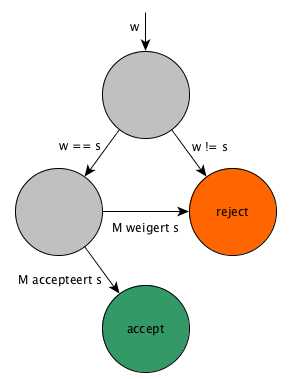
\includegraphics[width=0.3\textwidth]{./img/Ms}
  	\caption{Concept van $M_s$}
	\end{figure}
	Nu kunnen we verder met het bewijs. We proberen de stelling aan te tonen met een bewijs uit het ongerijmde. Stel dat $E_{TM}$ beslisbaar is en een beslisser $E$ heeft. We gaan nu een beslisser $B$ voor $A_{TM}$ opstellen met behulp van $E$\footnote{De beslisser $B$ kan niet bestaan, want $A_{TM}$ is onbeslisbaar. Dit wordt de contradictie.}. We kunnen twee punten inzien.
	\begin{enumerate}
		\item We stellen eerste onze hulpmachine $M_s$ op. We laten nu $E$ lopen over $<M_s>$. Stel dat $E$ nu $<M_s>$ accepteert. $M_s$ accepteert dus geen strings (zie definitie $E_{TM}$). Merk op dat in dit geval $B$ $<M,s>$ niet accepteert. $M_s$ bepaalt de lege taal, dus $M$ bepaalt $s$ niet.
		\item In het andere geval kan het zijn dat $E$ $<M_s>$ verwerpt. Dan bepaalt $M_s$ wel een taal (die niet leeg is) en zal dus $B$ zijn input wel accepteren.
	\end{enumerate}
	Uit bovenstaande punten kunnen we concluderen dat $E$ de tegenovergestelde uitkomst heeft van $B$. $B$ bestaat echter niet, aangezien $A_{TM}$ niet beslisbaar is. $E$ kan dus ook geen beslisser zijn en $E_{TM}$ is dus niet beslisbaar. Contradictie.
\end{proof}

\subsubsection*{$E_{TM}$ is niet herkenbaar maar wel co-herkenbaar}

\begin{proof}
	Het is makkelijk aan te tonen dat door eerst de co-herkenbaarheid van $E_{TM}$ te onderzoeken. Het complement van $E_{TM}$ bestaat uit alle Turingmachines die een niet lege taal bepalen. Neem nu Turingmachine $M \in \overline{E_{TM}}$ en dus $L_M \neq \phi$. We maken een hulpmachine die voor elk van die $M$ alle strings $s$ in de lexicografische volgorde $M$ laat lopen over $s$. Vanaf $M$ accepteert, accepteert de hulpmachine. Indien dit niet is, gaat hij verder met de volgende string $s$.
	Dit proces kan niet oneindig doorgaan, tenzij geen enkele string $s$ geaccepteerd wordt door $M$. $\overline{E_{TM}}$ is dus herkenbaar en dus is $E_{TM}$ co-herkenbaar.
	\\\\
	$E_{TM}$ is dus niet herkenbaar aangezien het co-herkenbaar is. Indien het ook herkenbaar is, zou het ook beslisbaar zijn. Dit is een contradictie met het vorige bewijs.
\end{proof}

\subsubsection*{Alternatieve bewijzen}

\begin{proof}
	Een alternatief bewijs zou kunnen zijn met behulp van de stelling van Rice. Een taal-invariante, niet-triviale eigenschap van $E_{TM}$ is dat $L_M = \phi$ voor elke $M$ in $E_{TM}$ die $L_M$ bepaalt. Volgens de stelling van Rice is $E_{TM}$ dus onbeslisbaar.
\end{proof}

\subsubsection*{Bespreek $E_{CFG}$}

\begin{theorem}
	$E_{CFG} = \{ <G> |$ $G$ \textit{is een} $CFG$, \textit{en} $L_G = \phi \}$ is beslisbaar: \textit{emptyness} van een $CFL$ is beslisbaar.
\end{theorem}

\begin{proof}
	We beschrijven formeel een algoritme dat $G$ transformeert naar een vorm waarin de beslissing gemakkelijk is.
	\begin{enumerate}
		\item Indien er een regel $A \rightarrow \alpha$ in zit en $\alpha$ bestaat alleen uit eindsymbolen (mag dus ook $\epsilon$ zijn), dan
		\begin{enumerate}
			\item Verwijder alle regels waar $A$ aan de linkerkant staat
			\item Vervang in elke regel waar $A$ rechts voorkomt, de voorkomens van $A$ voor $\alpha$
		\end{enumerate}
		\item Blijf dit doen totdat ofwel
		\begin{enumerate}
			\item Het startsymbool verwijderd is: reject, want het startsymbool kan een string afleiden.
			\item Er geen regels zijn van de benodigde vorm: accept, want de taal is leeg.
		\end{enumerate}
	\end{enumerate}
\end{proof}
